\documentclass[12pt,a4paper]{article}

\usepackage[
    left=20mm,
    right=10mm,
    top=20mm,
    bottom=12mm
]{geometry}

\usepackage[T1]{fontenc}
\usepackage[utf8]{inputenc}
\usepackage{lmodern}
\usepackage{graphicx}
\usepackage{xcolor}
\usepackage{fancyhdr}
\usepackage{caption}
\usepackage{tabularx}
\usepackage{xltabular}
\usepackage{array}
\usepackage{enumitem}
\usepackage{tikz}
\usetikzlibrary{shapes.geometric, positioning, calc, fit, arrows.meta}
\usepackage{pgfcalendar}
\usepackage{url}
\usepackage{hyperref}
\captionsetup[table]{position=bottom}

% -------------------------------------------------
% Page style
% -------------------------------------------------
\pagestyle{fancy}
\fancyhf{}
\fancyfoot[R]{\thepage}
\renewcommand{\headrulewidth}{0pt}
\renewcommand{\footrulewidth}{0pt}
\setlength{\footskip}{7mm}

% -------------------------------------------------
% Project information
% -------------------------------------------------
\newcommand{\ProjectHeading}{Group Project \textendash{} LAB 1, 2}

\newcommand{\ProjectTitle}{%
Design and Implementation of a Knowledge-Retrieval-Supported Application\\
for Creating Laboratory Assignments%
}

\newcommand{\ProjectAuthors}{Larisa Salamatova, Stanislaw Konariew}

\newcommand{\ProjectSupervisor}{%
Dr hab.\ inż.\ Jerzy Balicki, prof.\ PW%
}

\newcommand{\DocumentVersion}{version 1.1}
\newcommand{\DocumentDate}{19.10.2026}

% -------------------------------------------------
% Manual table-of-contents entry
% Usage: \TOCEntry{Title}{Page}
% Optional argument controls indentation.
% -------------------------------------------------
\newcommand{\TOCEntry}[3][0pt]{%
    \noindent
    \hspace*{#1}%
    \parbox[t]{0.80\textwidth}{#2}%
    \hfill
    #3\par
    \vspace{2mm}
}

% -------------------------------------------------
% UML stereotype in guillemets
% Usage: \guil{include}
% -------------------------------------------------
\newcommand{\guil}[1]{\guillemotleft#1\guillemotright}

% -------------------------------------------------
% Gantt chart helpers (project schedule)
% Dates are ISO (yyyy-mm-dd); \GanttOffset stores the number of
% days between \GanttSetOrigin and the given date in \GanttDay.
% -------------------------------------------------
\definecolor{ganttJoint}{HTML}{2A78D6}
\definecolor{ganttLarisa}{HTML}{EB6834}
\definecolor{ganttStanislaw}{HTML}{1BAF7A}
\definecolor{ganttInk}{HTML}{0B0B0B}
\definecolor{ganttMuted}{HTML}{52514E}
\definecolor{ganttGrid}{HTML}{E1E0D9}
\definecolor{ganttAxis}{HTML}{C3C2B7}

\newcommand{\GanttDayW}{1.08mm}
\newcommand{\GanttRowH}{6mm}

\newcount\GanttOrigin
\newcount\GanttDay
\newcommand{\GanttSetOrigin}[1]{\pgfcalendardatetojulian{#1}{\GanttOrigin}}
\newcommand{\GanttOffset}[1]{%
    \pgfcalendardatetojulian{#1}{\GanttDay}%
    \advance\GanttDay by -\GanttOrigin
}

% Usage: \GanttTask{row}{label}{first day}{last day}{colour}
\newcommand{\GanttTask}[5]{%
    \GanttOffset{#3}\edef\GanttFrom{\the\GanttDay}%
    \GanttOffset{#4}\advance\GanttDay by 1\relax
    \edef\GanttTo{\the\GanttDay}%
    \node[anchor=west] at (-62mm, {-(#1-0.5)*\GanttRowH}) {#1};
    \node[anchor=west] at (-57mm, {-(#1-0.5)*\GanttRowH}) {#2};
    \fill[#5, rounded corners=0.6mm]
        ({\GanttFrom*\GanttDayW}, {-(#1-0.5)*\GanttRowH+1.8mm})
        rectangle
        ({\GanttTo*\GanttDayW}, {-(#1-0.5)*\GanttRowH-1.8mm});
}

% Usage: \GanttMonth{first day}{first day of the next month}{label}
\newcommand{\GanttMonth}[3]{%
    \GanttOffset{#1}\edef\GanttFrom{\the\GanttDay}%
    \GanttOffset{#2}\edef\GanttTo{\the\GanttDay}%
    \node at ({(\GanttFrom+\GanttTo)/2*\GanttDayW}, 7mm) {#3};
    \draw[ganttAxis] ({\GanttTo*\GanttDayW}, 9.5mm) --
        ({\GanttTo*\GanttDayW}, -81mm);
}

% Usage: \GanttMilestone{due date}{label}; drawn at the end of the day
\newcommand{\GanttMilestone}[2]{%
    \GanttOffset{#1}\advance\GanttDay by 1\relax
    \edef\GanttAt{\the\GanttDay}%
    \node[gantt milestone] at ({\GanttAt*\GanttDayW}, -75mm) {};
    \node[font=\scriptsize] at ({\GanttAt*\GanttDayW}, -78.6mm) {#2};
}

\begin{document}

% =================================================
% Page 1 -- Cover page
% =================================================
\thispagestyle{fancy}

\begin{figure}[t]
    \centering
    % The document still compiles if the logo file is unavailable.
    \IfFileExists{logo cover page.png}{%
        \includegraphics[width=\linewidth]{logo cover page.png}%
    }{%
        \vspace*{10mm}%
    }
\end{figure}

\vspace*{45mm}

\begin{center}
    {\Large\bfseries \ProjectHeading\par}

    \vspace{5mm}

    {\Large \ProjectTitle\par}

    \vspace{25mm}

    {\large \ProjectAuthors\par}

    \vspace{10mm}

    {\normalsize Supervisor: \ProjectSupervisor\par}

    \vspace{35mm}

    {\large \DocumentVersion\par}

    \vspace{15mm}

    {\large \DocumentDate\par}
\end{center}

\clearpage

% =================================================
% Page 2 -- Table of contents
% =================================================
\thispagestyle{fancy}

\begin{center}
    {\Large\bfseries Table of Contents\par}
\end{center}

\vspace{8mm}

% Page numbers come from the \label commands in each section,
% so they update automatically when the layout changes.
\TOCEntry{1 Abstract}{\pageref{sec:abstract}}
\TOCEntry[1em]{1.1 History of changes}{\pageref{sec:history}}
\TOCEntry{2 Vocabulary}{\pageref{sec:vocabulary}}
\TOCEntry{3 Specification}{\pageref{sec:specification}}
\TOCEntry[1em]{3.1 Executive summary}{\pageref{sec:executive-summary}}
\TOCEntry[1em]{3.2 Functional requirements}{\pageref{sec:functional-requirements}}
\TOCEntry[1em]{3.3 Non-functional requirements}{\pageref{sec:nonfunctional-requirements}}
\TOCEntry{4 Project schedule}{\pageref{sec:schedule}}
\TOCEntry{5 Risk Analysis}{\pageref{sec:risk}}
\TOCEntry{6 System Architecture and Design}{\pageref{sec:architecture}}
\TOCEntry{7 Justification of Technology Stack Choice}{\pageref{sec:technology-stack}}
\TOCEntry{8 API Contracts}{\pageref{sec:api-contracts}}
\TOCEntry{9 Planned Database Schema (Relational ERD)}{\pageref{sec:database-schema}}
\TOCEntry{10 Bibliography}{\pageref{sec:bibliography}}

\clearpage

% =================================================
% Page 3 -- Abstract
% =================================================
\thispagestyle{fancy}

\noindent
{\Large\bfseries\textcolor{blue!55!black}{1 Abstract}\par}
\label{sec:abstract}

\vspace{12mm}

The aim of this work is to design, implement, and evaluate a configurable web application that supports creation of laboratory assignments for academic courses using Retrieval-Augmented Generation (RAG).

The application will generate structured, evidence-grounded assignments from user-provided course materials according to configurable pedagogical requirements. The solution will be evaluated using Operating Systems course materials as a case study through a reproducible comparative analysis of baseline vector RAG, Hybrid RAG, LightRAG, and GraphRAG with respect to retrieval relevance, source traceability, factual correctness, learning outcome alignment, latency and estimated inference cost.

For GraphRAG, evaluate whether relation type, relation weight, and graph-centrality measures improve assignment structuring compared with the baseline: concepts identified as central or pedagogically essential shall be candidates for core tasks, while concepts connected through weaker or supporting relations shall be candidates for prerequisites, contextual explanations, hints, or optional extensions.

The outcome will be a documented and deployable web application for instructors, together with a reproducible evaluation benchmark, automated test suite, experiment configurations and aggregated evaluation results.

\clearpage


% =================================================
% History of changes
% =================================================
\setcounter{section}{1}
\setcounter{subsection}{0}

\subsection{History of changes}
\label{sec:history}
\thispagestyle{fancy}

\begin{table}[htbp]
    \centering
    \renewcommand{\arraystretch}{1.4}
    \begin{tabularx}{\textwidth}{|p{25mm}|p{20mm}|p{45mm}|X|}
        \hline
        \textbf{Date} &
        \textbf{Version} &
        \textbf{Author} &
        \textbf{Description of changes} \\
        \hline
        19.10.2026 &
        1.0 &
        Larisa Salamatova, Stanislaw Konariew &
        Initial version of the laboratory project report. \\
        \hline
        19.10.2026 &
        1.1 &
        Larisa Salamatova, Stanislaw Konariew &
        Abstract, Vocabulary, Specification, Project Schedule,
        Risk Analysis, and Bibliography. \\
        \hline
        28.10.2026 &
        1.2 &
        Stanislaw Konariew &
        System Architecture and Design\\
        \hline
        28.10.2026 &
        1.2 &
        Larisa Salamatova &
        Justification of Technology Stack Choice\\
        \hline
        30.10.2026 &
        1.3 &
        Larisa Salamatova, Stanislaw Konariew &
        API Contracts, Planned Database Schema\\
        \hline
    \end{tabularx}
    \caption{History of Changes}
    \label{tab:history-changes}
\end{table}

\clearpage

% =================================================
% 2 Vocabulary
% =================================================
\section{Vocabulary}
\label{sec:vocabulary}

\begin{description}[style=nextline,leftmargin=0pt,labelindent=0pt]

\item[Retrieval-Augmented Generation (RAG)]
A technique that combines information retrieval with text generation.
Relevant passages are retrieved from a knowledge collection and
provided to a language model as contextual evidence for generating
a response. In this project, RAG is used to support the creation of
laboratory assignments grounded in approved course materials
\cite{lewis2020rag}.

\item[Knowledge base]
A collection of documents and associated metadata used as the
permitted source of information for retrieval. The application will
maintain a primary knowledge base for authoritative materials from
the target course and a supplementary knowledge base for approved
materials from related or earlier courses.

\item[Corpus]
The set of documents selected for processing and evaluation.
The project corpus will consist of permitted course materials
selected according to documented inclusion and exclusion rules.

\item[Document ingestion]
The process of importing source documents, extracting their text,
assigning metadata, segmenting the content, and preparing it for
indexing and retrieval. The planned supported formats are PDF,
HTML, TXT, and Markdown.

\item[Chunking]
The process of dividing a document into smaller text segments.
These segments are indexed and retrieved as contextual evidence.
Each indexed segment must retain its source identifier and a
retrievable text excerpt.

\item[Embedding]
A numerical vector representation of text used to identify
semantically related content. Embeddings will support the baseline
vector retrieval pipeline.

\item[Vector retrieval]
A retrieval method that searches indexed vector representations
for passages relevant to a query. It is the baseline retrieval
approach against which the alternative architectures will be
evaluated.

\item[Hybrid retrieval]
A retrieval approach combining complementary retrieval methods,
such as lexical matching and vector similarity, to retrieve
potentially relevant passages.

\item[LightRAG]
A retrieval-augmented generation approach that incorporates
knowledge representations and graph-based retrieval techniques
\cite{guo2024lightrag}. It will be evaluated as one of the
alternative retrieval architectures in this project.

\item[GraphRAG]
A RAG approach that uses a graph representation of entities and
their relationships to support retrieval and generation
\cite{edge2024graphrag}. This project will investigate whether
relation types, relation weights, and graph-centrality measures
can improve the structure of generated assignments.

\item[Metadata]
Descriptive information associated with a document or indexed
fragment. Planned metadata fields include knowledge-base type,
course, document type, topic, version, learning outcomes,
difficulty level, and authority level, where available.

\item[Source traceability]
The ability to identify the source document and supporting text
for a generated claim or mandatory assignment requirement.
The application will retain links between generated content
and retrieved evidence.

\item[Learning outcome]
A statement describing the knowledge or competence a student
should acquire through a course or learning activity. Generated
assignments will be configured to support specified learning
outcomes.

\item[Held-out benchmark]
A fixed collection of evaluation requests reserved for testing
the compared architectures. The benchmark will be defined before
architecture tuning and will not be used for prompt development,
configuration tuning, or architecture selection.

\item[Evidence coverage]
The extent to which substantive technical claims and mandatory
task requirements are supported by retrieved source excerpts.

\item[Unsupported claim]
A claim for which the retrieved evidence does not provide
adequate support. The project will also distinguish contradicted
claims from claims that are merely unsupported.

\item[CI/CD]
Continuous integration and continuous delivery or deployment.
In this project, the CI workflow automatically runs quality
checks, tests, and a Docker image build for pull requests
targeting the main branch.

\item[Docker]
A containerization platform used to package software and its
runtime environment. The current repository includes a Dockerfile
for building the Python project image.

\item[uv]
A Python project and dependency management tool used to create
the development environment, install dependencies, and support
reproducible installations.

\end{description}

\clearpage

% =================================================
% 3 Specification
% =================================================
\section{Specification}
\label{sec:specification}

\subsection{Executive summary}
\label{sec:executive-summary}

The purpose of this project is to design and implement a
configurable web application that supports instructors in creating
laboratory assignments from approved academic course materials.
The application will use Retrieval-Augmented Generation (RAG)
to provide language models with relevant evidence retrieved from
a closed, course-specific knowledge base.

The initial case study will use Operating Systems course materials.
The solution will maintain separate primary and supplementary
knowledge bases. Primary-course materials will be authoritative
for mandatory technical requirements, course-specific tools,
learning outcomes, and assessment criteria. Supplementary
materials may provide prerequisites, contextual explanations,
hints, and optional extensions, but must not override primary
sources.

The project will compare baseline vector RAG, Hybrid RAG,
LightRAG, and GraphRAG under a common evaluation protocol.
The comparison will consider retrieval relevance, source
traceability, factual correctness, learning-outcome alignment,
latency, and estimated inference cost, among other metrics.

The generated assignments will follow a configurable structure
including a title, prerequisites, objectives, environment and
tools, tasks, submission requirements, assessment rubric, and
source evidence. The system will validate generated output before
presenting it as a complete assignment.

The final deliverable will include a documented and deployable
web application, automated tests, reproducible experiment
configurations and scripts, a held-out benchmark, evaluation
rubrics, and aggregated evaluation results.

At the time of this specification, the repository provides the
Python development environment, dependency management,
testing setup, code-quality checks, Docker configuration, and
GitHub Actions workflow. The RAG implementation and application
layer remain planned work and must not be considered implemented
features.

\subsection{Functional requirements}
\label{sec:functional-requirements}

The following user-oriented requirements describe the intended
capabilities of the completed system.

As an instructor or project administrator, I would like to:

\begin{itemize}
    \item Import permitted PDF, HTML, TXT, and Markdown course
    documents and manage their metadata. (Must have)

    \item Maintain separate primary and supplementary knowledge
    bases. (Must have)

    \item Extract, segment, index, and retrieve document content
    while preserving source identifiers and excerpts. (Must have)

    \item Configure assignment topics, learning outcomes,
    difficulty levels, course stages, target competencies,
    expected duration, and assignment format. (Must have)

    \item Generate structured laboratory assignments using
    evidence retrieved from the approved knowledge bases.
    (Must have)

    \item Inspect the evidence supporting generated claims and
    mandatory task requirements. (Must have)

    \item Validate assignment structure, source references,
    and evidence coverage before presenting a complete result.
    (Must have)

    \item Receive a structured explanation when evidence is
    missing, contradictory, or insufficient. (Must have)

    \item Edit individual assignment sections and regenerate
    selected sections. (Should have)

    \item Export generated assignments for further use.
    (Should have)

    \item Compare the evaluated retrieval architectures and
    reproduce experiments using saved configurations.
    (Must have for project evaluation)

    \item Review aggregated evaluation results, including
    retrieval quality, factual correctness, latency, and cost.
    (Must have for project evaluation)
\end{itemize}

\subsubsection*{Detailed functional requirements}

% xltabular (longtable + tabularx) lets this table break across
% pages; the header row is repeated on every continuation page.
\begingroup
\small
\renewcommand{\arraystretch}{1.3}
\begin{xltabular}{\textwidth}{
    |p{12mm}|p{28mm}|p{36mm}|X|
}
\hline
\textbf{ID} &
\textbf{Actor} &
\textbf{Name} &
\textbf{Description and expected response} \\
\hline
\endfirsthead

\hline
\textbf{ID} &
\textbf{Actor} &
\textbf{Name} &
\textbf{Description and expected response} \\
\hline
\endhead

\multicolumn{4}{r}{\textit{Continued on the next page}} \\
\endfoot

\caption{Detailed functional requirements}
\label{tab:functional-requirements} \\
\endlastfoot

FR-01 &
Instructor &
Document management &
The system shall allow users to import permitted documents
in PDF, HTML, TXT, and Markdown formats and inspect their
associated metadata. \\
\hline

FR-02 &
System administrator &
Knowledge-base separation &
The system shall maintain primary and supplementary knowledge
bases and apply the configured source-authority policy during
retrieval and generation. \\
\hline

FR-03 &
Application &
Ingestion and indexing &
The system shall extract text, assign available metadata,
segment documents, and create searchable indexes. Each
indexed fragment shall retain a source identifier and
retrievable text excerpt. \\
\hline

FR-04 &
Instructor &
Assignment configuration &
The system shall accept topic, learning outcomes, difficulty,
course stage, target competencies, expected duration, and
assignment format as configuration parameters. \\
\hline

FR-05 &
Application &
Evidence retrieval &
The system shall retrieve relevant passages from the approved
knowledge bases using the selected retrieval architecture and
configured retrieval parameters. \\
\hline

FR-06 &
Instructor &
Assignment generation &
The system shall generate assignments containing a title,
prerequisites, objectives, environment and tools, tasks,
submission requirements, an assessment rubric, and source
evidence. \\
\hline

FR-07 &
Application &
Source traceability &
Each substantive technical claim and mandatory task
requirement shall be linked to at least one retrieved source
excerpt and its source-document identifier. \\
\hline

FR-08 &
Application &
Output validation &
The system shall validate the output schema, required sections,
source-reference validity, and evidence coverage of mandatory
requirements before presenting a complete assignment. \\
\hline

FR-09 &
Application &
Insufficient or conflicting evidence &
If required evidence is unavailable, contradictory, or fails
validation, the system shall return a structured response
explaining the reason instead of presenting a complete
assignment. \\
\hline

FR-10 &
Instructor &
Assignment editing &
The system should allow section-level editing and regeneration
of selected assignment sections. \\
\hline

FR-11 &
Instructor &
Export &
The system should allow a generated assignment to be exported
in a suitable format for instructors. The exact export formats
will be defined during implementation. \\
\hline

FR-12 &
Researcher &
Architecture comparison &
The system shall support reproducible evaluation of baseline
vector RAG, Hybrid RAG, LightRAG, and GraphRAG using a common
benchmark and evaluation protocol. \\
\hline

FR-13 &
Researcher &
Experiment records &
The system shall retain benchmark requests, experiment
configurations, execution logs, and evaluation results
required for reproducibility. \\
\hline

FR-14 &
Researcher &
Evaluation reporting &
The system shall support reporting of retrieval, evidence,
generation-quality, performance, and estimated-cost metrics. \\
\hline

FR-15 &
Development team &
Automated testing &
The project shall provide automated tests for ingestion,
metadata filtering, source traceability, validation,
unsupported requests, conflicting evidence, and repeated
generation scenarios. \\
\hline

\end{xltabular}
\endgroup

\subsubsection*{Use cases}

The principal actors and their interactions with the planned
application are summarized below.

\begin{table}[htbp]
\centering
\small
\renewcommand{\arraystretch}{1.3}
\begin{tabularx}{\textwidth}{|p{35mm}|X|}
\hline
\textbf{Actor} & \textbf{Use cases} \\
\hline
Instructor &
Manage course materials and metadata, prepare the corpus and
indexes, configure official assignments, generate, edit, and
regenerate official assignments, inspect supporting evidence
and validation results, and export official assignments. \\
\hline
Student &
Configure and generate practice assignments, inspect learning
evidence and source references, and save or export practice
assignments. \\
\hline
Researcher / Administrator &
Manage experiment configurations and retrieval parameters,
prepare benchmark requests, run architecture comparisons,
review evaluation results, and select the standard retrieval
architecture. \\
\hline
Development team &
Run automated tests, check code quality, build the Docker image,
and maintain the continuous-integration workflow. \\
\hline
\end{tabularx}
\caption{Actors and use cases}
\label{tab:use-cases}
\end{table}

\subsubsection*{Student practice mode}

Students use the application in a dedicated practice mode, in
which they can configure and generate practice assignments,
inspect the supporting evidence and source references, and save
or export the result. The mode does not permit students to
modify the corpus, metadata, source-authority policy, official
assignment configurations, or instructor-only materials. Its
purpose is to support self-directed preparation for laboratory
classes by identifying relevant concepts, prerequisites, and
course sources.

\subsubsection*{Use-case diagram}

The following diagram presents the main interactions with
the planned application. It represents intended functionality,
not the current implementation state. Use-case priorities follow
the MoSCoW scheme (Must, Should, Could); dashed arrows denote
\guil{include} and \guil{extend} relationships.

\begin{figure}[htbp]
\centering
% Scaled down only if wider than the text block; otherwise natural size.
\resizebox{\ifdim\width>\linewidth\linewidth\else\width\fi}{!}{%
\begin{tikzpicture}[
    font=\fontsize{9}{10.5}\selectfont,
    pics/stickman/.style={
        code={
            \draw (0,4.2mm) circle[radius=1.8mm];
            \draw (0,2.4mm) -- (0,-1.8mm);
            \draw (-3mm,1mm) -- (3mm,1mm);
            \draw (0,-1.8mm) -- (-2.6mm,-6mm);
            \draw (0,-1.8mm) -- (2.6mm,-6mm);
        }
    },
    actor/.style={
        minimum width=6mm,
        minimum height=12mm,
        inner sep=0pt
    },
    usecase/.style={
        draw,
        ellipse,
        align=center,
        inner sep=1pt,
        minimum width=42mm,
        minimum height=15mm
    },
    dep/.style={
        draw,
        dashed,
        -{Straight Barb[length=1.8mm]}
    },
    rel/.style={
        font=\scriptsize,
        inner sep=1pt
    }
]
    % Distances are measured between node borders,
    % so the ellipses cannot overlap.

    % Right column: student (top) and researcher (bottom) use cases.
    \node[usecase] (s1)
        {\textit{\guil{Should}}\\Configure practice\\assignment};
    \node[usecase, below=5mm of s1] (s2)
        {\textit{\guil{Should}}\\Generate practice\\assignment};
    \node[usecase, below=5mm of s2] (s3)
        {\textit{\guil{Should}}\\Inspect learning\\evidence and source\\references};
    \node[usecase, below=5mm of s3] (s4)
        {\textit{\guil{Could}}\\Save or export\\practice assignment};
    \node[usecase, below=9mm of s4] (s5)
        {\textit{\guil{Must}}\\Manage experiment\\configurations};
    \node[usecase, below=5mm of s5] (s6)
        {\textit{\guil{Must}}\\Run architecture\\comparison};
    \node[usecase, below=5mm of s6] (s7)
        {\textit{\guil{Must}}\\Review evaluation\\results};

    % Left column: instructor use cases, shifted down to centre
    % the column against the right one.
    \coordinate (lc) at ($(s1.north)+(-60mm,-10mm)$);
    \node[usecase, anchor=north] (l1) at (lc)
        {\textit{\guil{Must}}\\Manage course\\materials and\\metadata};
    \node[usecase, below=5mm of l1] (l2)
        {\textit{\guil{Must}}\\Prepare corpus\\and indexes};
    \node[usecase, below=5mm of l2] (l3)
        {\textit{\guil{Must}}\\Configure official\\assignment};
    \node[usecase, below=5mm of l3] (l4)
        {\textit{\guil{Must}}\\Generate, edit, and\\regenerate official\\assignment};
    \node[usecase, below=5mm of l4] (l5)
        {\textit{\guil{Must}}\\Inspect evidence\\and validation};
    \node[usecase, below=5mm of l5] (l6)
        {\textit{\guil{Should}}\\Export official\\assignment};

    % System boundary with the title above the top row
    \coordinate (titlespace) at ($(s1.north)+(0,7mm)$);
    \node[
        draw,
        inner sep=4mm,
        fit=(titlespace)(l1)(l2)(l3)(l4)(l5)(l6)(s1)(s2)(s3)(s4)(s5)(s6)(s7),
        label={[anchor=north, font=\footnotesize\bfseries]north:RAG Laboratory Assignment Application}
    ] (system) {};

    % Actors, vertically centred on their own use cases. Labels sit
    % on the outer side so that association lines do not cross them.
    \coordinate (ipos) at ($(l3.west)!0.5!(l4.west)+(-15mm,0)$);
    \coordinate (spos) at ($(s2.east)!0.5!(s3.east)+(15mm,0)$);
    \coordinate (rpos) at ($(s6.east)+(15mm,0)$);
    \node[actor, label={[anchor=north east, align=right]south east:Instructor}]
        (instructor) at (ipos) {};
    \node[actor, label={[anchor=north west, align=left]south west:Student}]
        (student) at (spos) {};
    \node[actor, label={[anchor=north west, align=left]south west:Researcher /\\Administrator}]
        (researcher) at (rpos) {};
    \foreach \a in {instructor, student, researcher}
        \pic at (\a) {stickman};

    % Associations end at the outer tips of the ellipses, so they
    % never pass through neighbouring use cases.
    \foreach \uc in {l1, l2, l3, l4, l5, l6}
        \draw (instructor.east) -- (\uc.west);
    \foreach \uc in {s1, s2, s3, s4}
        \draw (student.west) -- (\uc.east);
    \foreach \uc in {s5, s6, s7}
        \draw (researcher.west) -- (\uc.east);

    % Include and extend relationships
    \draw[dep] (l4) -- node[rel, right] {\guil{include}} (l3);
    \draw[dep] (l5) -- node[rel, right] {\guil{extend}} (l4);
    \draw[dep] (l6.east) to[out=0, in=0, looseness=0.7]
        node[rel, fill=white] {\guil{extend}} (l4.east);
    \draw[dep] (s2) -- node[rel, right] {\guil{include}} (s1);
    \draw[dep] (s3) -- node[rel, right] {\guil{extend}} (s2);
    \draw[dep] (s4.west) to[out=180, in=180, looseness=0.7]
        node[rel, fill=white] {\guil{extend}} (s2.west);
    \draw[dep] (s6) -- node[rel, right] {\guil{include}} (s5);

    % Legend
    \node[draw, rounded corners=2pt, anchor=north east, font=\scriptsize, inner sep=2mm]
        at ($(system.south east)+(0,-4mm)$)
        {\begin{tabular}{@{}l@{\quad}l@{}}
            \textit{\guil{Must}}   & core functionality \\
            \textit{\guil{Should}} & next priority \\
            \textit{\guil{Could}}  & nice to have
        \end{tabular}};
\end{tikzpicture}%
}
\caption{Use cases of the planned RAG laboratory assignment application}
\label{fig:use-case-diagram}
\end{figure}

\subsection{Non-functional requirements}
\label{sec:nonfunctional-requirements}

The following non-functional requirements define quality,
reproducibility, and operational expectations for the completed
system. Requirements involving measurable performance will be
evaluated experimentally; numerical acceptance thresholds must
be defined before the relevant experiments.

\begin{table}[htbp]
\centering
\small
\renewcommand{\arraystretch}{1.3}
\begin{tabularx}{\textwidth}{|p{12mm}|p{33mm}|X|}
\hline
\textbf{ID} &
\textbf{Area} &
\textbf{Requirement} \\
\hline

NFR-01 &
Reliability &
The system shall handle unsupported file formats, extraction
errors, and invalid input through controlled error responses. \\
\hline

NFR-02 &
Traceability &
Generated technical claims and mandatory task requirements
shall retain references to source excerpts and source-document
identifiers. \\
\hline

NFR-03 &
Factual correctness &
The system shall validate generated content against retrieved
evidence and avoid presenting an assignment as complete when
required evidence is missing, contradictory, or invalid. \\
\hline

NFR-04 &
Educational quality &
Generated assignments shall be assessed for alignment with
specified learning outcomes and for educational usefulness
using a predefined expert-assessment rubric. \\
\hline

NFR-05 &
Reproducibility &
The benchmark, experiment configurations, corpus rules,
evaluation scripts, and relevant execution records shall be
retained to support repeatable comparisons. \\
\hline

NFR-06 &
Comparability &
The compared retrieval architectures shall use the same corpus,
generation model, prompt template, output schema, validation
procedure, benchmark, and evaluation protocol, except for
documented experimental variations. \\
\hline

NFR-07 &
Security &
Secrets such as API keys shall be supplied through environment
configuration and shall not be committed to the repository
or copied into the Docker image. \\
\hline

NFR-08 &
Maintainability &
The codebase shall use consistent formatting and linting
checks, automated tests, dependency management, and a
documented feature-branch and pull-request workflow. \\
\hline

NFR-09 &
Deployability &
The project shall provide a Docker image build and documented
instructions for installing dependencies and configuring
the application. \\
\hline

NFR-10 &
Performance &
The evaluation shall measure retrieval and generation latency,
indexing time, storage use, token usage, and estimated
inference cost. Acceptance thresholds will be set based on
the evaluation environment and project requirements. \\
\hline

NFR-11 &
Evaluation integrity &
The held-out benchmark shall contain at least 60 requests,
with at least 8 requests in each specified evaluation category,
and shall not be used for prompt development, configuration
tuning, or architecture selection. \\
\hline

NFR-12 &
Evidence validation &
The evidence-validation mechanism shall be evaluated on a
manually annotated subset of at least 60 generated claims,
reporting precision, recall, and F1-score for supported,
contradicted, and unsupported classifications. \\
\hline

\end{tabularx}
\caption{Non-functional requirements}
\label{tab:nonfunctional-requirements}
\end{table}

The evaluation shall also report unsupported-claim rates before
and after validation. The final architecture shall be selected
according to a predefined decision rule that prioritizes
grounding, factual correctness, and learning-outcome alignment
while considering operational cost.

\clearpage

% =================================================
% 4 Project schedule
% =================================================
\section{Project schedule}
\label{sec:schedule}

The project schedule is a provisional plan covering the period
from 1~October 2026 to 15~January 2027. It reflects the proposed
division of work and the dependency between corpus preparation,
evaluation design, retrieval implementation, application
development, and final validation.

The initial repository infrastructure includes dependency
management, a smoke test, code-quality checks, Docker
configuration, and a GitHub Actions workflow. The status of
these components should be confirmed against the actual
repository before final submission.

\begin{table}[htbp]
\centering
\small
\renewcommand{\arraystretch}{1.25}
\begin{tabularx}{\textwidth}{
    |p{8mm}|X|p{32mm}|p{21mm}|p{21mm}|p{18mm}|
}
\hline
\textbf{No.} &
\textbf{Task} &
\textbf{Responsible member(s)} &
\textbf{Start} &
\textbf{End} &
\textbf{Status} \\
\hline

1 &
Project planning, thesis requirements, and repository setup &
Larisa, Stanislaw &
01.10.2026 &
25.10.2026 &
In progress* \\
\hline

2 &
Corpus selection, permitted-source rules, and metadata design &
Larisa, Stanislaw &
26.10.2026 &
08.11.2026 &
Planned \\
\hline

3 &
Benchmark design, evaluation metrics, and expert rubric &
Stanislaw &
26.10.2026 &
15.11.2026 &
Planned \\
\hline

4 &
Persistent storage, document ingestion, chunking, and indexing &
Larisa, Stanislaw &
02.11.2026 &
22.11.2026 &
Planned \\
\hline

5 &
Baseline vector RAG pipeline and retrieval configuration &
Larisa &
16.11.2026 &
29.11.2026 &
Planned \\
\hline

6 &
Hybrid RAG, LightRAG, and GraphRAG implementation &
Larisa, Stanislaw &
30.11.2026 &
20.12.2026 &
Planned \\
\hline

7 &
Assignment generation, evidence linking, and validation &
Larisa &
23.11.2026 &
13.12.2026 &
Planned \\
\hline

8 &
Instructor-facing web application and export &
Larisa, Stanislaw &
07.12.2026 &
03.01.2027 &
Planned \\
\hline

9 &
Automated tests and evidence-validation evaluation &
Stanislaw &
30.11.2026 &
03.01.2027 &
Planned \\
\hline

10 &
Comparative experiments and results analysis &
Stanislaw, Larisa &
21.12.2026 &
10.01.2027 &
Planned \\
\hline

11 &
Deployment, documentation, and reproducibility checks &
Larisa, Stanislaw &
28.12.2026 &
10.01.2027 &
Planned \\
\hline

12 &
Final report, review, and presentation preparation &
Larisa, Stanislaw &
04.01.2027 &
15.01.2027 &
Planned \\
\hline
\end{tabularx}
\caption{Provisional project schedule}
\label{tab:project-schedule}
\end{table}

\noindent
\textit{* The initial planning and repository setup are described
in the project README. Confirm which tasks have actually been
completed before assigning their final status. The dates above
are proposed estimates and should be adjusted to the official
submission schedule.}

\medskip
\noindent
Figure~\ref{fig:gantt-chart} presents the same schedule as a Gantt
chart. Bar colours indicate the responsible team members, and the
diamonds mark the milestones listed below.

\begin{figure}[htbp]
\centering
% Scaled down only if wider than the text block; otherwise natural size.
\resizebox{\ifdim\width>\linewidth\linewidth\else\width\fi}{!}{%
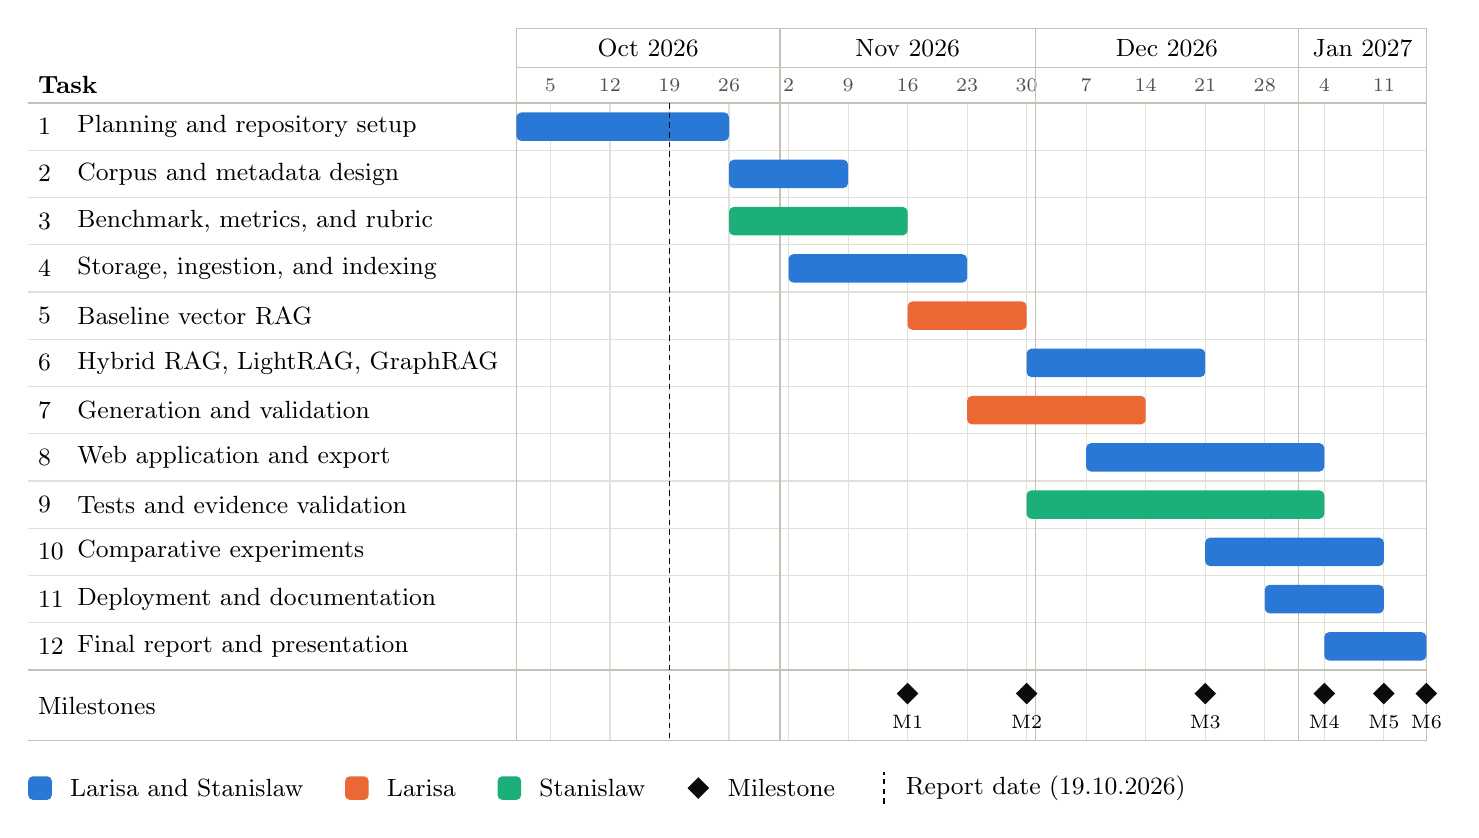
\begin{tikzpicture}[
    font=\fontsize{9}{11}\selectfont,
    gantt swatch/.style={
        rounded corners=0.6mm,
        minimum width=3mm,
        minimum height=3mm,
        inner sep=0pt
    },
    gantt milestone/.style={
        diamond,
        fill=ganttInk,
        minimum size=2.8mm,
        inner sep=0pt
    },
    gantt today/.style={
        draw=ganttInk,
        dash pattern=on 2pt off 1.5pt,
        line width=0.6pt
    }
]
    % Time axis: 01.10.2026 to 15.01.2027 inclusive (107 days)
    \GanttSetOrigin{2026-10-01}
    \GanttOffset{2027-01-16}\edef\GanttEnd{\the\GanttDay}
    \def\GanttRight{\GanttEnd*\GanttDayW}

    % Week grid: one line per Monday, labelled with its day of month
    % (\x is the day offset from 01.10.2026)
    \foreach \x/\dom in {4/5, 11/12, 18/19, 25/26, 32/2, 39/9, 46/16,
                         53/23, 60/30, 67/7, 74/14, 81/21, 88/28,
                         95/4, 102/11} {
        \draw[ganttGrid] (\x*\GanttDayW, 0) -- (\x*\GanttDayW, -81mm);
        \node[font=\scriptsize, text=ganttMuted]
            at (\x*\GanttDayW, 2.25mm) {\dom};
    }

    % Row separators
    \foreach \y in {1,...,11}
        \draw[ganttGrid] (-62mm, -\y*\GanttRowH) --
            (\GanttRight, -\y*\GanttRowH);

    % Header and frame
    \draw[ganttAxis] (0, 9.5mm) -- (\GanttRight, 9.5mm);
    \draw[ganttAxis] (0, 4.5mm) -- (\GanttRight, 4.5mm);
    \draw[ganttAxis] (-62mm, 0) -- (\GanttRight, 0);
    \draw[ganttAxis] (-62mm, -72mm) -- (\GanttRight, -72mm);
    \draw[ganttAxis] (-62mm, -81mm) -- (\GanttRight, -81mm);
    \draw[ganttAxis] (0, 9.5mm) -- (0, -81mm);
    \node[anchor=west, font=\fontsize{9}{11}\selectfont\bfseries]
        at (-62mm, 2.25mm) {Task};

    \GanttMonth{2026-10-01}{2026-11-01}{Oct 2026}
    \GanttMonth{2026-11-01}{2026-12-01}{Nov 2026}
    \GanttMonth{2026-12-01}{2027-01-01}{Dec 2026}
    \GanttMonth{2027-01-01}{2027-01-16}{Jan 2027}

    % Tasks (numbers and dates as in the schedule table)
    \GanttTask{1}{Planning and repository setup}{2026-10-01}{2026-10-25}{ganttJoint}
    \GanttTask{2}{Corpus and metadata design}{2026-10-26}{2026-11-08}{ganttJoint}
    \GanttTask{3}{Benchmark, metrics, and rubric}{2026-10-26}{2026-11-15}{ganttStanislaw}
    \GanttTask{4}{Storage, ingestion, and indexing}{2026-11-02}{2026-11-22}{ganttJoint}
    \GanttTask{5}{Baseline vector RAG}{2026-11-16}{2026-11-29}{ganttLarisa}
    \GanttTask{6}{Hybrid RAG, LightRAG, GraphRAG}{2026-11-30}{2026-12-20}{ganttJoint}
    \GanttTask{7}{Generation and validation}{2026-11-23}{2026-12-13}{ganttLarisa}
    \GanttTask{8}{Web application and export}{2026-12-07}{2027-01-03}{ganttJoint}
    \GanttTask{9}{Tests and evidence validation}{2026-11-30}{2027-01-03}{ganttStanislaw}
    \GanttTask{10}{Comparative experiments}{2026-12-21}{2027-01-10}{ganttJoint}
    \GanttTask{11}{Deployment and documentation}{2026-12-28}{2027-01-10}{ganttJoint}
    \GanttTask{12}{Final report and presentation}{2027-01-04}{2027-01-15}{ganttJoint}

    % Milestones
    \node[anchor=west] at (-62mm, -76.5mm) {Milestones};
    \GanttMilestone{2026-11-15}{M1}
    \GanttMilestone{2026-11-29}{M2}
    \GanttMilestone{2026-12-20}{M3}
    \GanttMilestone{2027-01-03}{M4}
    \GanttMilestone{2027-01-10}{M5}
    \GanttMilestone{2027-01-15}{M6}

    % Report date
    \GanttOffset{2026-10-19}\edef\GanttAt{\the\GanttDay}
    \draw[gantt today] (\GanttAt*\GanttDayW, 0) -- (\GanttAt*\GanttDayW, -81mm);

    % Legend
    \node[gantt swatch, fill=ganttJoint] (k1) at (-60.5mm, -87mm) {};
    \node[anchor=west] (t1) at ([xshift=1mm]k1.east) {Larisa and Stanislaw};
    \node[gantt swatch, fill=ganttLarisa, right=4mm of t1] (k2) {};
    \node[anchor=west] (t2) at ([xshift=1mm]k2.east) {Larisa};
    \node[gantt swatch, fill=ganttStanislaw, right=4mm of t2] (k3) {};
    \node[anchor=west] (t3) at ([xshift=1mm]k3.east) {Stanislaw};
    \node[gantt milestone, right=4mm of t3] (k4) {};
    \node[anchor=west] (t4) at ([xshift=1mm]k4.east) {Milestone};
    \coordinate (k5) at ([xshift=5mm]t4.east);
    \draw[gantt today] ($(k5)+(0,-2mm)$) -- ($(k5)+(0,2mm)$);
    \node[anchor=west] at ([xshift=1.5mm]k5) {Report date (19.10.2026)};
\end{tikzpicture}%
}
\caption{Gantt chart of the provisional project schedule}
\label{fig:gantt-chart}
\end{figure}

\subsection*{Milestones}

\begin{itemize}
    \item M1 (by 15.11.2026): Approved corpus, source-authority
    policy, and frozen held-out benchmark.

    \item M2 (by 29.11.2026): Persistent storage, ingestion,
    metadata, and baseline vector retrieval working.

    \item M3 (by 20.12.2026): All four retrieval architectures
    available for controlled comparison.

    \item M4 (by 03.01.2027): Assignment generation and evidence
    validation integrated into the web application.

    \item M5 (by 10.01.2027): Automated tests and comparative
    evaluation completed.

    \item M6 (by 15.01.2027): Deployable application, reproducible
    artifacts, documentation, and final report prepared.
\end{itemize}

\clearpage

% =================================================
% 5 Risk analysis
% =================================================
\section{Risk Analysis}
\label{sec:risk}

The following analysis identifies internal strengths and
weaknesses, external opportunities and threats, and the main
risks that may affect successful completion of the project.
The likelihood ratings are preliminary qualitative estimates
and should be reviewed as development progresses.

\subsection{Strengths (Internal)}

\begin{itemize}
    \item A defined thesis objective and a detailed proposal
    describing the intended application and evaluation protocol.

    \item A Python development setup with dependency management
    through \texttt{uv}.

    \item A repository structure that separates source code
    and tests.

    \item Automated code-quality checks and a smoke-test setup.

    \item Docker configuration and a GitHub Actions workflow
    for repeatable build and test checks.

    \item A clear division of responsibilities between the
    two team members.
\end{itemize}

\subsection{Weaknesses (Internal)}

\begin{itemize}
    \item The RAG implementation and application layer have
    not yet been included in the repository.

    \item The project requires implementation and comparison
    of four retrieval architectures.

    \item The evaluation requires a manually prepared benchmark,
    source annotations, and expert assessment.

    \item The quality of results depends on consistent corpus
    preparation, metadata, prompts, and validation rules.

    \item The project has a limited development period of
    approximately three and a half months (October 2026 --
    mid-January 2027).
\end{itemize}

\subsection{Opportunities (External)}

\begin{itemize}
    \item Academic supervision and feedback from the thesis
    supervisor.

    \item Availability of published research on RAG, retrieval
    evaluation, and graph-based retrieval approaches
    \cite{lewis2020rag,guo2024lightrag,edge2024graphrag,
    salemi2024retrieval}.

    \item Potential usefulness of evidence-grounded assignment
    generation for instructors preparing laboratory classes.

    \item A reproducible benchmark and evaluation framework
    that may support further research.

    \item An opportunity to produce a documented software
    project suitable for a development portfolio.
\end{itemize}

\subsection{Threats (External)}

\begin{itemize}
    \item Changes in the availability, pricing, or behaviour
    of external language-model and embedding APIs.

    \item Restrictions on access to course materials or
    permission to use particular documents.

    \item Changes in third-party libraries or incompatibilities
    between software dependencies.

    \item Limited availability of experts to assess generated
    assignments and manually annotate claims.

    \item Hardware limitations or API rate limits affecting
    the time and cost required to run comparative experiments.
\end{itemize}

\subsection{Main risks and mitigation measures}

\begin{table}[htbp]
\centering
\small
\renewcommand{\arraystretch}{1.3}
\begin{tabularx}{\textwidth}{|p{29mm}|p{18mm}|X|}
\hline
\textbf{Risk} &
\textbf{Likelihood} &
\textbf{Mitigation measures} \\
\hline

Implementation complexity &
Likely &
Implement the baseline pipeline first, separate components
into modules, define interfaces early, and prioritize
mandatory requirements before optional features. \\
\hline

Insufficient corpus quality &
Possible &
Define inclusion and exclusion rules, preserve source
metadata, verify extracted text, and document missing or
inaccessible source materials. \\
\hline

Benchmark contamination &
Possible &
Freeze the benchmark before tuning, restrict its use to
evaluation, record experiment configurations, and document
any deviations from the protocol. \\
\hline

Unsupported or incorrect generated claims &
Likely &
Require claim-to-evidence links, validate mandatory
requirements, test unsupported and conflicting requests,
and report validation precision, recall, and F1-score. \\
\hline

API cost or rate limits &
Possible &
Record token usage and estimated cost, apply request limits,
cache reusable results where appropriate, and schedule
experiments within a documented budget. \\
\hline

Non-reproducible comparisons &
Possible &
Keep the corpus, generation model, prompts, output schema,
validation procedure, benchmark, and evaluation environment
consistent across architectures, documenting deviations. \\
\hline

Dependency or deployment failures &
Possible &
Use a lock file, run automated checks in CI, build the
Docker image regularly, and test the documented setup
instructions. \\
\hline

Schedule delays &
Likely &
Define milestones, monitor progress, allocate time for
integration and debugging, and prioritize the required
evaluation and final deliverables. \\
\hline

\end{tabularx}
\caption{Principal project risks and mitigation measures}
\label{tab:project-risks}
\end{table}

\clearpage
% =================================================
% LAB02 START
% =================================================

\section{System Architecture and Design}
\label{sec:architecture}
\subsection{System architecture: modules and their responsibilities}
\subsection{Modules design: interfaces dependencies, layers}
\subsection{Communication Layer Design: protocols, libraries, network}
\subsection{Main components description: classes, states, activity, events diagrams}
\subsection{User interface vision: schemes, plots, drawings}
\subsection{External interfaces: standards, file formats, norms}

\section{Justification of Technology Stack Choice}
\label{sec:technology-stack}

The application uses Python 3.12 and \texttt{uv} for its runtime and
dependency management, FastAPI for its HTTP API, PostgreSQL for
relational application data, and Chroma for persistent vector
retrieval. React provides the instructor-facing web interface.
Redis and RQ handle long-running ingestion, indexing, and evaluation
jobs. Docker Compose coordinates the application services for local
deployment. The same generation and embedding model configuration
is used across retrieval architectures during comparative
evaluation.

\begingroup
\small
\renewcommand{\arraystretch}{1.3}
\begin{xltabular}{\textwidth}{
    |p{25mm}|p{38mm}|p{34mm}|X|
}
\hline
\textbf{Module / Component} &
\textbf{Selected Technology} &
\textbf{Considered Alternatives} &
\textbf{Justification and Trade-offs} \\
\hline
\endfirsthead

\hline
\textbf{Module / Component} &
\textbf{Selected Technology} &
\textbf{Considered Alternatives} &
\textbf{Justification and Trade-offs} \\
\hline
\endhead

\multicolumn{4}{r}{\textit{Continued on the next page}} \\
\endfoot

\caption{Technology stack for the RAG laboratory assignment application}
\label{tab:technology-stack} \\
\endlastfoot

Runtime and dependency management &
\textbf{Python 3.12 and \texttt{uv}} &
Python with Poetry; Python with \texttt{pip} and \texttt{venv} &
Python 3.12 is the version used by the repository's CI and Docker
image, and \texttt{uv} with a lock file supports repeatable
dependency installation. The trade-off is reliance on an additional
tool in the development workflow. \\
\hline

Backend API &
\textbf{FastAPI} &
Flask; Django &
FastAPI fits the selected Python runtime, supports typed request
and response validation, and generates an OpenAPI interface useful
for the web client and experiments. It adds a framework dependency;
asynchronous endpoints do not by themselves accelerate CPU-bound
indexing or model inference. \\
\hline

Relational application database &
\textbf{PostgreSQL} &
SQLite; MongoDB &
The application must persist related records for documents,
metadata, assignments, claim-to-evidence links, benchmark requests,
experiment configurations, logs, and results. PostgreSQL provides
transactional relational storage for these records. It requires a
separate service and more setup than SQLite; a document database
would make these relationships and consistency rules less direct. \\
\hline

Vector store &
\textbf{Chroma persistent storage} &
PostgreSQL with \texttt{pgvector}; FAISS &
A persistent vector index supports the baseline retrieval pipeline
and local course-specific corpora. Keeping it separate from
PostgreSQL means source identifiers and metadata must be
synchronized and both stores must be backed up. \\
\hline

Generation and embeddings &
\textbf{OpenAI API with configurable model IDs} &
Other hosted model APIs; locally hosted models &
Configurable model identifiers support a controlled comparison of
vector RAG, Hybrid RAG, LightRAG, and GraphRAG using the same
generation and embedding models.
Hosted inference introduces API cost, network dependence, and
course-material data-governance considerations; keys must remain
outside source control and model usage must be recorded. \\
\hline

Background jobs &
\textbf{Redis and RQ} &
In-process tasks; Celery with RabbitMQ &
Document ingestion, indexing, and benchmark runs can outlast an
interactive web request. A worker queue lets the API submit these
jobs without blocking and allows their status to be tracked. Redis
adds an operational service; for a small prototype, in-process
execution is simpler but less suitable for durable, long-running
jobs. \\
\hline

Web interface &
\textbf{React, TypeScript, and Chart.js} &
Vue; Streamlit &
A component-based interface supports assignment configuration,
evidence inspection, section-level editing and regeneration, and
visualization of evaluation results. A separate JavaScript
application gives more control over these interactions but adds a
frontend build and maintenance stack; Streamlit would be simpler
for a Python-only prototype. \\
\hline

Testing &
\textbf{\texttt{pytest}} &
\texttt{unittest} &
\texttt{pytest} can cover ingestion formats, metadata filtering, traceability,
validation, unsupported requests, conflicting evidence, and
repeat-generation scenarios. \\
\hline

Deployment &
\textbf{Docker and Docker Compose} &
Direct installation; Kubernetes &
Docker packages the runtime, and Compose runs the API, worker,
PostgreSQL, and Redis together with persistent data volumes.
This supports reproducible deployment on a single lab machine;
Compose adds configuration to maintain and is not intended for
multi-node orchestration. \\
\hline

\end{xltabular}
\endgroup

\section{API Contracts (OpenAPI / Swagger Specification)}
\label{sec:api-contracts}

The HTTP API uses the \texttt{/api/v1} prefix and JSON request and
response bodies, except for document uploads, which use
\texttt{multipart/form-data}. FastAPI publishes the machine-readable
OpenAPI document at \texttt{/openapi.json}, the Swagger UI at
\texttt{/docs}, and the ReDoc interface at \texttt{/redoc}.
Protected endpoints require
\texttt{Authorization: Bearer \textless token\textgreater}. Authorization is
role-based: instructors manage course materials and assignments,
students may create and inspect practice assignments, and
researchers or administrators manage evaluation runs. Student
requests cannot modify course materials, metadata, or official
assignments.

\begingroup
\small
\renewcommand{\arraystretch}{1.25}
\begin{xltabular}{\textwidth}{
    |p{13mm}|p{65mm}|p{30mm}|X|
}
\hline
\textbf{Method} &
\textbf{Path} &
\textbf{Access} &
\textbf{Purpose and successful response} \\
\hline
\endfirsthead

\hline
\textbf{Method} &
\textbf{Path} &
\textbf{Access} &
\textbf{Purpose and successful response} \\
\hline
\endhead

\multicolumn{4}{r}{\textit{Continued on the next page}} \\
\endfoot

\caption{Version 1 application API endpoints}
\label{tab:api-endpoints} \\
\endlastfoot

GET &
\url{/api/v1/health} &
Public &
Returns service health and readiness. \texttt{200 OK}. \\
\hline

POST &
\url{/api/v1/documents} &
Instructor, administrator &
Uploads a PDF, HTML, TXT, or Markdown source with course and
authority metadata. Returns \texttt{202 Accepted} with a document
identifier and ingestion job identifier. \\
\hline

GET &
\url{/api/v1/documents} &
Instructor, administrator &
Lists documents with pagination and optional course,
knowledge-base, document-type, and ingestion-status filters.
Returns \texttt{200 OK}. \\
\hline

PATCH &
\url{/api/v1/documents/{document_id}/metadata} &
Instructor, administrator &
Updates document metadata without changing the source file.
Returns \texttt{200 OK}. \\
\hline

POST &
\url{/api/v1/courses/{course_id}/index} &
Instructor, administrator &
Indexes eligible primary and supplementary course materials
according to the source-authority policy. Returns
\texttt{202 Accepted} with a job identifier. \\
\hline

POST &
\url{/api/v1/assignments/generate} &
Instructor, student &
Starts assignment generation from the approved course knowledge
bases. Returns \texttt{202 Accepted} with a job identifier. \\
\hline

GET &
\url{/api/v1/jobs/{job_id}} &
Job owner, administrator &
Returns job status (\texttt{queued}, \texttt{running},
\texttt{succeeded}, or \texttt{failed}) and its result or
structured error. Returns \texttt{200 OK}. \\
\hline

GET &
\url{/api/v1/assignments/{assignment_id}} &
Assignment owner, instructor &
Returns assignment sections, configuration, validation state,
and claim-to-evidence links. Returns \texttt{200 OK}. \\
\hline

PATCH &
\url{/api/v1/assignments/{assignment_id}/sections/{section_id}} &
Instructor &
Edits a section and reruns the applicable validation checks.
Returns \texttt{200 OK} with the updated section and validation
result. \\
\hline

POST &
\url{/api/v1/assignments/{assignment_id}/sections/{section_id}/regenerate} &
Instructor &
Regenerates one section using the assignment configuration and
approved evidence. Returns \texttt{202 Accepted} with a job
identifier. \\
\hline

GET &
\url{/api/v1/assignments/{assignment_id}/export} &
Assignment owner, instructor &
Exports a validated assignment using the \texttt{format} query
parameter (\texttt{markdown} or \texttt{pdf}). Returns the file
with \texttt{200 OK}; an incomplete assignment returns
\texttt{409 Conflict}. \\
\hline

POST &
\url{/api/v1/evaluation-runs} &
Researcher, administrator &
Starts a reproducible run for a selected retrieval architecture
and frozen benchmark configuration. Returns \texttt{202 Accepted}
with a job identifier. \\
\hline

GET &
\url{/api/v1/evaluation-runs/{run_id}} &
Researcher, administrator &
Returns the run configuration, status, execution records, and
aggregated evaluation metrics. Returns \texttt{200 OK}. \\
\hline

\end{xltabular}
\endgroup

\subsection*{Document upload request}

The \texttt{POST /api/v1/documents} request uses
\texttt{multipart/form-data}. The \texttt{file} part contains the
source document, and the \texttt{metadata} part contains JSON:

\begin{verbatim}
{
  "course_id": "operating-systems",
  "knowledge_base": "primary",
  "document_type": "lecture_notes",
  "topic": "process_synchronization",
  "version": "2026",
  "learning_outcomes": ["LO-3"],
  "authority_level": "course"
}
\end{verbatim}

The \texttt{knowledge\_base} value is either \texttt{primary} or
\texttt{supplementary}. The primary knowledge base is authoritative
for mandatory technical requirements, course tools, learning
outcomes, and assessment criteria. Supplementary sources may
support prerequisites, context, hints, and optional extensions.
The response is \texttt{202 Accepted}:

\begin{verbatim}
{
  "document_id": "1c3645c2-9b91-4a2d-b91e-98b401301111",
  "ingestion_status": "queued",
  "job_id": "7ebf9105-0eb7-4a4b-83b8-2e5abc89d222"
}
\end{verbatim}

\subsection*{Assignment generation request}

The \texttt{POST /api/v1/assignments/generate} request accepts the
pedagogical configuration required by the assignment specification:

\begin{verbatim}
{
  "course_id": "operating-systems",
  "topic": "process synchronization",
  "learning_outcomes": ["LO-3"],
  "difficulty": "intermediate",
  "course_stage": "after-lectures-5-6",
  "target_competencies": ["concurrency"],
  "expected_duration_minutes": 120,
  "assignment_format": "individual_lab"
}
\end{verbatim}

The server selects the default retrieval architecture for standard
use. Evaluation runs select an architecture through their saved
experiment configuration. The generation request returns
\texttt{202 Accepted}:

\begin{verbatim}
{
  "job_id": "8e20742d-96c8-4f4f-9ea1-a7ea8d7e3333",
  "status": "queued",
  "status_url": "/api/v1/jobs/8e20742d-96c8-4f4f-9ea1-a7ea8d7e3333"
}
\end{verbatim}

Clients poll the status URL. A successful job result contains an
assignment identifier and a validation state. An assignment is
marked \texttt{complete} only when its required
sections, source references, and mandatory evidence checks pass.
Missing, contradicted, or unsupported evidence is returned as a
structured validation issue and the assignment is marked
\texttt{incomplete}.

\subsection*{Assignment and validation response}

The \texttt{GET /api/v1/assignments/\{assignment\_id\}} response
includes the required assignment sections and evidence links. Each
evidence item identifies the source document, indexed fragment, and
retrievable excerpt. Claim-level evidence identifiers refer to
entries in \texttt{source\_evidence}. A successful response has
this structure:

\begin{verbatim}
{
  "assignment_id": "9f31853e-a7d9-4c54-8fb2-b8fb94aa4444",
  "status": "complete",
  "sections": {
    "title": "Process Synchronization",
    "prerequisites": ["Processes and threads"],
    "objectives": ["Apply synchronization primitives"],
    "environment_and_tools": ["Approved course environment"],
    "tasks": [
      {
        "section_id": "a042964f-b7f2-4c17-8e80-c9c3d6bb5555",
        "title": "Analyze a race condition",
        "description": "Identify the shared state and propose a fix.",
        "mandatory": true,
        "claims": [
          {
            "claim_id": "b153a750-c803-4d28-9f91-dad4e7cc6666",
            "text": "The task uses concepts introduced in the course.",
            "support_status": "supported",
            "evidence_ids": ["c264b861-d914-4e39-a0a2-ebe5f8dd7777"]
          }
        ]
      }
    ],
    "submission_requirements": ["Submit the report and source code"],
    "assessment_rubric": [
      {
        "criterion": "Correctness",
        "description": "The solution addresses the race condition.",
        "weight": 100
      }
    ]
  },
  "source_evidence": [
    {
      "evidence_id": "c264b861-d914-4e39-a0a2-ebe5f8dd7777",
      "document_id": "1c3645c2-9b91-4a2d-b91e-98b401301111",
      "fragment_id": "d375c972-ea25-4f4a-b1b3-fcf609ee8888",
      "knowledge_base": "primary",
      "excerpt": "Relevant text from the approved course material."
    }
  ],
  "validation": {
    "status": "passed",
    "issues": []
  }
}
\end{verbatim}

When required evidence is missing, contradicted, or unsupported,
the affected claim or requirement is returned as a structured
validation issue classified as \texttt{unsupported},
\texttt{contradicted}, or \texttt{missing\_evidence}. The assignment
is marked \texttt{incomplete} and cannot be exported as a validated
assignment. For example:

\begin{verbatim}
{
  "assignment_id": "9f31853e-a7d9-4c54-8fb2-b8fb94aa4444",
  "status": "incomplete",
  "validation": {
    "status": "blocked",
    "issues": [
      {
        "code": "MISSING_PRIMARY_EVIDENCE",
        "section_id": "tasks",
        "claim": "Use the specified course tool",
        "classification": "missing_evidence",
        "message": "No primary-course source supports this requirement."
      }
    ]
  }
}
\end{verbatim}

\subsection*{Error responses}

Errors use a consistent JSON envelope containing a stable error
code, a human-readable message, and optional field or evidence
details. The API returns \texttt{400 Bad Request} for malformed
requests, \texttt{401 Unauthorized} for missing or invalid
credentials, \texttt{403 Forbidden} for insufficient role access,
\texttt{404 Not Found} for unknown resources, \texttt{409 Conflict}
for invalid state transitions or incomplete-assignment export,
\texttt{413 Payload Too Large} for oversized uploads,
\texttt{415 Unsupported Media Type} for unsupported document
formats, and \texttt{422 Unprocessable Entity} for schema or
business-rule validation failures.

\begin{verbatim}
{
  "error": {
    "code": "UNSUPPORTED_DOCUMENT_FORMAT",
    "message": "The uploaded file type is not supported.",
    "details": {
      "accepted_formats": ["pdf", "html", "txt", "md"]
    },
    "request_id": "req_01J8ZC20"
  }
}
\end{verbatim}

% =================================================
% 9 Planned Database Schema
% =================================================
\section{Planned Database Schema (Relational ERD)}
\label{sec:database-schema}

PostgreSQL stores users, course and source metadata, extracted
document fragments, assignments, evidence links, benchmark
requests, experiment configurations, job states, and evaluation
results. Original source files are stored in persistent file
storage. Chroma stores vector embeddings and indexes; each
relational document-fragment record stores the corresponding
Chroma collection and record identifiers. Foreign keys preserve
the relationships between courses, knowledge bases, documents,
fragments, generated claims, and supporting evidence.

\begin{verbatim}
-- User accounts and application roles
CREATE TABLE users (
    user_id UUID PRIMARY KEY,
    email VARCHAR(320) NOT NULL UNIQUE,
    display_name VARCHAR(128) NOT NULL,
    user_role VARCHAR(20) NOT NULL CHECK (
        user_role IN ('instructor', 'student', 'researcher', 'administrator')
    ),
    created_at TIMESTAMPTZ NOT NULL DEFAULT CURRENT_TIMESTAMP
);

-- Courses and their primary or supplementary knowledge bases
CREATE TABLE courses (
    course_id VARCHAR(64) PRIMARY KEY,
    name VARCHAR(256) NOT NULL,
    created_at TIMESTAMPTZ NOT NULL DEFAULT CURRENT_TIMESTAMP
);

CREATE TABLE knowledge_bases (
    knowledge_base_id UUID PRIMARY KEY,
    course_id VARCHAR(64) NOT NULL REFERENCES courses(course_id)
        ON DELETE CASCADE,
    knowledge_base_role VARCHAR(20) NOT NULL CHECK (
        knowledge_base_role IN ('primary', 'supplementary')
    ),
    name VARCHAR(256) NOT NULL,
    created_at TIMESTAMPTZ NOT NULL DEFAULT CURRENT_TIMESTAMP,
    UNIQUE (course_id, knowledge_base_role)
);

-- Source metadata and the location of the original file
CREATE TABLE source_documents (
    document_id UUID PRIMARY KEY,
    knowledge_base_id UUID NOT NULL
        REFERENCES knowledge_bases(knowledge_base_id),
    uploaded_by UUID REFERENCES users(user_id),
    filename VARCHAR(512) NOT NULL,
    media_type VARCHAR(128) NOT NULL,
    storage_uri TEXT NOT NULL UNIQUE,
    checksum_sha256 CHAR(64),
    metadata JSONB NOT NULL DEFAULT '{}'::JSONB,
    ingestion_status VARCHAR(20) NOT NULL DEFAULT 'queued'
        CHECK (ingestion_status IN (
            'queued', 'processing', 'indexed', 'failed'
        )),
    error_message TEXT,
    created_at TIMESTAMPTZ NOT NULL DEFAULT CURRENT_TIMESTAMP,
    updated_at TIMESTAMPTZ NOT NULL DEFAULT CURRENT_TIMESTAMP
);

-- Extracted text fragments and their corresponding Chroma records
CREATE TABLE document_chunks (
    chunk_id UUID PRIMARY KEY,
    document_id UUID NOT NULL
        REFERENCES source_documents(document_id) ON DELETE CASCADE,
    chunk_index INTEGER NOT NULL CHECK (chunk_index >= 0),
    content TEXT NOT NULL,
    page_number INTEGER CHECK (page_number IS NULL OR page_number > 0),
    section_path TEXT[] NOT NULL DEFAULT '{}',
    metadata JSONB NOT NULL DEFAULT '{}'::JSONB,
    chroma_collection VARCHAR(256) NOT NULL,
    chroma_record_id VARCHAR(256) NOT NULL,
    created_at TIMESTAMPTZ NOT NULL DEFAULT CURRENT_TIMESTAMP,
    UNIQUE (document_id, chunk_index),
    UNIQUE (chroma_collection, chroma_record_id)
);

-- Generated official and practice assignments
CREATE TABLE assignments (
    assignment_id UUID PRIMARY KEY,
    course_id VARCHAR(64) NOT NULL REFERENCES courses(course_id),
    owner_id UUID NOT NULL REFERENCES users(user_id),
    mode VARCHAR(16) NOT NULL CHECK (mode IN ('official', 'practice')),
    status VARCHAR(16) NOT NULL CHECK (
        status IN ('generating', 'complete', 'incomplete', 'failed')
    ),
    validation_status VARCHAR(16) NOT NULL DEFAULT 'pending'
        CHECK (validation_status IN ('pending', 'passed', 'blocked')),
    retrieval_architecture VARCHAR(20) NOT NULL CHECK (
        retrieval_architecture IN ('vector', 'hybrid', 'lightrag', 'graphrag')
    ),
    configuration JSONB NOT NULL,
    created_at TIMESTAMPTZ NOT NULL DEFAULT CURRENT_TIMESTAMP,
    updated_at TIMESTAMPTZ NOT NULL DEFAULT CURRENT_TIMESTAMP,
    CHECK (status <> 'complete' OR validation_status = 'passed'),
    CHECK (status <> 'incomplete' OR validation_status = 'blocked')
);

-- Structured assignment sections; repeated task sections use position
CREATE TABLE assignment_sections (
    section_id UUID PRIMARY KEY,
    assignment_id UUID NOT NULL
        REFERENCES assignments(assignment_id) ON DELETE CASCADE,
    section_key VARCHAR(32) NOT NULL CHECK (
        section_key IN (
            'title', 'prerequisites', 'objectives',
            'environment_and_tools', 'tasks',
            'submission_requirements', 'assessment_rubric'
        )
    ),
    position INTEGER NOT NULL DEFAULT 0 CHECK (position >= 0),
    content JSONB NOT NULL,
    updated_at TIMESTAMPTZ NOT NULL DEFAULT CURRENT_TIMESTAMP,
    UNIQUE (assignment_id, section_key, position)
);

-- Substantive claims and their support classification
CREATE TABLE generated_claims (
    claim_id UUID PRIMARY KEY,
    section_id UUID NOT NULL
        REFERENCES assignment_sections(section_id) ON DELETE CASCADE,
    claim_text TEXT NOT NULL,
    claim_type VARCHAR(32) NOT NULL CHECK (
        claim_type IN ('technical', 'mandatory_requirement', 'other')
    ),
    support_status VARCHAR(16) NOT NULL CHECK (
        support_status IN (
            'pending', 'supported', 'contradicted', 'unsupported'
        )
    ),
    is_mandatory BOOLEAN NOT NULL DEFAULT FALSE,
    created_at TIMESTAMPTZ NOT NULL DEFAULT CURRENT_TIMESTAMP
);

-- Claim-to-source links; the cited excerpt remains in document_chunks
CREATE TABLE claim_evidence (
    evidence_id UUID PRIMARY KEY,
    claim_id UUID NOT NULL
        REFERENCES generated_claims(claim_id) ON DELETE CASCADE,
    chunk_id UUID NOT NULL
        REFERENCES document_chunks(chunk_id),
    relation VARCHAR(16) NOT NULL CHECK (
        relation IN ('supports', 'contradicts', 'context')
    ),
    UNIQUE (claim_id, chunk_id, relation)
);

-- Frozen benchmark sets and their evaluation requests
CREATE TABLE benchmark_sets (
    benchmark_set_id UUID PRIMARY KEY,
    name VARCHAR(256) NOT NULL,
    version VARCHAR(64) NOT NULL,
    split VARCHAR(16) NOT NULL CHECK (
        split IN ('development', 'held_out')
    ),
    frozen_at TIMESTAMPTZ,
    created_at TIMESTAMPTZ NOT NULL DEFAULT CURRENT_TIMESTAMP,
    UNIQUE (name, version),
    CHECK (split <> 'held_out' OR frozen_at IS NOT NULL)
);

CREATE TABLE benchmark_requests (
    request_id UUID PRIMARY KEY,
    benchmark_set_id UUID NOT NULL
        REFERENCES benchmark_sets(benchmark_set_id) ON DELETE CASCADE,
    course_id VARCHAR(64) NOT NULL REFERENCES courses(course_id),
    category VARCHAR(32) NOT NULL CHECK (
        category IN (
            'single_source', 'multi_source', 'supplementary',
            'unsupported', 'conflicting', 'difficulty_or_stage'
        )
    ),
    request_payload JSONB NOT NULL,
    expected_evidence JSONB NOT NULL DEFAULT '[]'::JSONB,
    expected_outcome JSONB NOT NULL DEFAULT '{}'::JSONB,
    created_at TIMESTAMPTZ NOT NULL DEFAULT CURRENT_TIMESTAMP
);

-- Reproducible architecture comparisons and their measured results
CREATE TABLE evaluation_runs (
    run_id UUID PRIMARY KEY,
    benchmark_set_id UUID NOT NULL
        REFERENCES benchmark_sets(benchmark_set_id),
    created_by UUID NOT NULL REFERENCES users(user_id),
    architecture VARCHAR(20) NOT NULL CHECK (
        architecture IN ('vector', 'hybrid', 'lightrag', 'graphrag')
    ),
    generation_model VARCHAR(256) NOT NULL,
    embedding_model VARCHAR(256) NOT NULL,
    prompt_version VARCHAR(64) NOT NULL,
    output_schema_version VARCHAR(64) NOT NULL,
    validation_version VARCHAR(64) NOT NULL,
    configuration JSONB NOT NULL,
    status VARCHAR(16) NOT NULL CHECK (
        status IN ('queued', 'running', 'succeeded', 'failed')
    ),
    started_at TIMESTAMPTZ,
    completed_at TIMESTAMPTZ,
    created_at TIMESTAMPTZ NOT NULL DEFAULT CURRENT_TIMESTAMP
);

CREATE TABLE evaluation_metrics (
    run_id UUID NOT NULL
        REFERENCES evaluation_runs(run_id) ON DELETE CASCADE,
    metric_name VARCHAR(64) NOT NULL,
    dimension VARCHAR(64) NOT NULL DEFAULT 'overall',
    metric_value DOUBLE PRECISION NOT NULL,
    sample_count INTEGER CHECK (sample_count IS NULL OR sample_count >= 0),
    details JSONB NOT NULL DEFAULT '{}'::JSONB,
    PRIMARY KEY (run_id, metric_name, dimension)
);

-- Queue state and execution logs
CREATE TABLE background_jobs (
    job_id UUID PRIMARY KEY,
    rq_job_id VARCHAR(256) NOT NULL UNIQUE,
    job_type VARCHAR(32) NOT NULL CHECK (
        job_type IN (
            'document_ingestion', 'course_indexing',
            'assignment_generation', 'section_regeneration',
            'evaluation'
        )
    ),
    status VARCHAR(16) NOT NULL CHECK (
        status IN ('queued', 'running', 'succeeded', 'failed')
    ),
    requested_by UUID NOT NULL REFERENCES users(user_id),
    course_id VARCHAR(64) REFERENCES courses(course_id),
    document_id UUID REFERENCES source_documents(document_id),
    assignment_id UUID REFERENCES assignments(assignment_id),
    run_id UUID REFERENCES evaluation_runs(run_id),
    error_code VARCHAR(64),
    error_message TEXT,
    created_at TIMESTAMPTZ NOT NULL DEFAULT CURRENT_TIMESTAMP,
    started_at TIMESTAMPTZ,
    completed_at TIMESTAMPTZ,
    CHECK (
        num_nonnulls(course_id, document_id, assignment_id, run_id) = 1
    )
);

CREATE TABLE execution_logs (
    log_id BIGINT GENERATED ALWAYS AS IDENTITY PRIMARY KEY,
    job_id UUID NOT NULL
        REFERENCES background_jobs(job_id) ON DELETE CASCADE,
    level VARCHAR(16) NOT NULL CHECK (
        level IN ('debug', 'info', 'warning', 'error')
    ),
    event_type VARCHAR(64) NOT NULL,
    message TEXT NOT NULL,
    details JSONB NOT NULL DEFAULT '{}'::JSONB,
    recorded_at TIMESTAMPTZ NOT NULL DEFAULT CURRENT_TIMESTAMP
);

-- Common query paths
CREATE INDEX idx_documents_knowledge_base
    ON source_documents(knowledge_base_id, ingestion_status);
CREATE INDEX idx_documents_metadata
    ON source_documents USING GIN (metadata);
CREATE INDEX idx_knowledge_bases_course
    ON knowledge_bases(course_id);
CREATE INDEX idx_chunks_document
    ON document_chunks(document_id, chunk_index);
CREATE INDEX idx_chunks_metadata
    ON document_chunks USING GIN (metadata);
CREATE INDEX idx_assignments_owner_created
    ON assignments(owner_id, created_at DESC);
CREATE INDEX idx_assignment_sections_assignment
    ON assignment_sections(assignment_id, section_key, position);
CREATE UNIQUE INDEX idx_assignment_single_sections
    ON assignment_sections(assignment_id, section_key)
    WHERE section_key <> 'tasks';
CREATE INDEX idx_claims_section
    ON generated_claims(section_id);
CREATE INDEX idx_claim_evidence_chunk
    ON claim_evidence(chunk_id);
CREATE INDEX idx_jobs_status_created
    ON background_jobs(status, created_at DESC);
CREATE INDEX idx_benchmark_requests_set
    ON benchmark_requests(benchmark_set_id, category);
CREATE INDEX idx_evaluation_runs_benchmark
    ON evaluation_runs(benchmark_set_id, created_at DESC);
CREATE INDEX idx_execution_logs_job_time
    ON execution_logs(job_id, recorded_at);
\end{verbatim}

% =================================================
% 10 Bibliography
% =================================================
\section{Bibliography}
\label{sec:bibliography}

\begin{thebibliography}{9}

\bibitem{lewis2020rag}
P. Lewis et al.,
``Retrieval-Augmented Generation for Knowledge-Intensive NLP Tasks,''
in \textit{Advances in Neural Information Processing Systems},
vol. 33, 2020.
Available:
\url{https://proceedings.neurips.cc/paper_files/paper/2020/hash/6b493230205f780e1bc26945df7481e5-Abstract.html}.

\bibitem{guo2024lightrag}
Z. Guo, L. Xia, Y. Yu, T. Ao, and C. Huang,
``LightRAG: Simple and Fast Retrieval-Augmented Generation,''
arXiv preprint arXiv:2410.05779, 2024.
doi: 10.48550/arXiv.2410.05779.
Available: \url{https://doi.org/10.48550/arXiv.2410.05779}.

\bibitem{li2025bestpractices}
S. Li, L. Stenzel, C. Eickhoff, and S. A. Bahrainian,
``Enhancing Retrieval-Augmented Generation: A Study of Best Practices,''
arXiv preprint arXiv:2501.07391, 2025.
doi: 10.48550/arXiv.2501.07391.
Available: \url{https://doi.org/10.48550/arXiv.2501.07391}.

\bibitem{salemi2024retrieval}
A. Salemi and H. Zamani,
``Evaluating Retrieval Quality in Retrieval-Augmented Generation,''
in \textit{Proceedings of the 47th International ACM SIGIR Conference
on Research and Development in Information Retrieval},
2024, pp. 2395--2400.
doi: 10.1145/3626772.3657957.
Available: \url{https://doi.org/10.1145/3626772.3657957}.

\bibitem{edge2024graphrag}
D. Edge et al.,
``From Local to Global: A Graph RAG Approach to Query-Focused
Summarization,''
arXiv preprint arXiv:2404.16130, 2024.
Available: \url{https://arxiv.org/abs/2404.16130}.

\end{thebibliography}

\end{document}
